\documentclass[answers]{exam}

\usepackage[dvipsnames]{xcolor}
\usepackage{amsmath}
\usepackage{amsfonts}
\usepackage{amsthm}
\usepackage{microtype}
\usepackage{siunitx}
\DeclareSIUnit\year{yr}
\usepackage{pgfplots}
\usepackage{graphicx}
\usepackage{sidecap}
\sidecaptionvpos{figure}{c}
\usepackage{float}
\usepackage{gensymb}
\usepackage{tkz-euclide}
\usetkzobj{all}
\usepackage{commath}

\newtheorem*{thm}{Theorem}

\renewcommand*{\thefootnote}{\fnsymbol{footnote}}

% russian integral
\usepackage{scalerel}
\DeclareMathOperator*{\rint}{\scalerel*{\rotatebox{17}{$\!\int\!$}}{\int}}

% \qformat{Question \thequestion: \thequestiontitle\hfill}

\begin{document}

\section*{NCEA Level 2 Physics\\Assignment M4: Revision}
This assignment is entirely made up of questions that cover precisely the material
that you \textbf{need} to know for the mechanics topic. Thus, unlike the earlier
assignments, I expect this one (a) to requre less deep thinking on your part, and
(b) to be done completely.
It is a little longer than the other assignments as well: since none of the questions
should require any clever thinking, you should be able to get through them faster
than normal.

Several of the questions ask for explanations; what you are being marked on is clarity
and understanding. That is, you need to write clearly and precisely (using correct English grammar, and
with minimum waffling).

\paragraph{Example.} \emph{State the law of conservation of momentum.} The law of conservation
of momentum states that if no external forces act on a system then the total momentum of
the objects in that system does not change.


\begin{center}
{\color{red}\large{\textbf{Draw diagrams and explain your reasoning!!!}}}\end{center}

\subsection*{Part A}
Short answer questions --- you should be able to do all of these without too much
thought. If you find any of them difficult, please let me know so we can revise the
relevant material.
\begin{questions}
  \question A stone is thrown straight up with an initial speed of \SI{20}{\metre\per\second}.
            If the only force acting on it is gravity:
    \begin{parts}
      \part How high does the stone go?
      \part How long does it take to reach that maximum height?
    \end{parts}
  \question How large a horizontal force must be exerted on a \SI{920}{\kilo\gram} car in order
            to give it an acceleration of \SI{3.0}{\metre\per\second\squared} along a flat road,
            assuming that friction is negligible?
  \question What net force must act on a \SI{950}{\kilo\gram} car to accelerate it from rest
            to a speed of \SI{60}{\kilo\metre\per\hour} in \SI{8.0}{\second}?
  \question State the law of conservation of energy.
  \question A piano, mass \SI{270}{\kilo\gram}, is dropped from a window \SI{12.0}{\metre}
            above the ground.
    \begin{parts}
      \part What speed is it travelling when it hits the roof of a car \SI{170}{\centi\metre}
            above the ground?
      \part What is the momentum of the piano at the instant of impact?
      \part How long did the piano take to fall?
    \end{parts}
  \question It is found experimentally that a force of \SI{4.9}{\newton} is needed to extend
            a spring by \SI{0.05}{\metre} from its equilibrium position. The spring is then hung
            vertically with an unknown mass attached to the end, and the extension from equilibrium
            length is measured to be \SI{27}{\centi\metre}. Assume the spring is massless.
    \begin{parts}
      \part Draw a force diagram, showing all the forces acting on the mass.
      \part What is the size of the mass?
    \end{parts}
  \question A merry-go-round is observed to take \SI{360}{\second} to complete a full rotation. The
            radius of the merry-go-round is \SI{5}{\metre}.
    \begin{parts}
      \part Zavana is sitting on the edge of the spinning disc. How fast is she travelling?
      \part Calculate the centripetal force felt by Zavana, if she has a mass of \SI{65}{\kilo\gram}.
    \end{parts}
\end{questions}

\clearpage
\subsection*{Part B}
Long answer questions --- in order to pass this standard at merit/excellence level,
you must be able to do all of these problems.
\begin{questions}
  \question \textit{Circular motion.} The earth is orbiting the sun at a constant speed, in a roughly circular orbit.
    \begin{parts}
      \part Explain, with physical arguments, why the net force on the earth must be directed
            towards the centre of the sun.
      \part The earth has mass \SI{5.97e24}{\kilo\gram}, orbits the sun once every year (365.25 days),
            and is on average a distance \SI{1.496e11}{\metre} from the centre of the sun. Calculate
            the strength of the gravity force exerted \textbf{on the earth} by the sun.
      \part What is the strength and direction of the gravity force exerted \textbf{on the sun} by the earth?
    \end{parts}
  \question \textit{Energy.} Many swimming pools have diving boards. Suppose such a board is fixed at one end, and the board
            is flexible (so if a person sits on other the end it bends down). Mark (mass: \SI{74}{\kilo\gram}) is
            sitting on the end of a diving board, \SI{2.0}{\metre} away from the fixed pivot point. We can
            model the end of the flexible diving board as a spring that roughly follows Hooke's law.
    \begin{parts}
      \part State Hooke's law.
      \part If the end of the diving board has dipped down by \SI{2.5}{\centi\metre} from the horizontal,
            calculate the spring constant of the board.
      \part Mark jumps into the air and lands back on the board; the board is now dipping \SI{3.4}{\centi\metre}
            from the horizontal. How high \textbf{above the equilibrium point of the board} did Mark jump?
      \part Some of the energy which enabled Mark to jump to this height came from the elasticity of the board.
            How much \textbf{additional} work $ K $ did Mark have to do in order to reach this height?
      \part Mark now jumps again, this time landing in the water. He is travelling at a speed of \SI{20}{\metre\per\second}
            when he hits the water. Assuming that the energy which enabled this jump came from the two same sources
            as before --- the elastic energy of the board and a new input of energy $ K' $ by Mark --- calculate
            the height of the equilibrium point of the board above the water.
    \end{parts}
  \question \textit{Forces.} I pull a trolley of mass \SI{20}{\kilo\gram} along the ground at a constant speed of \SI{5}{\metre\per\second}.
            The handle of the trolley makes an angle \SI{30}{\degree} with the horizontal.
    \begin{parts}
      \part State the magnitude and direction of the \textbf{net} force on the trolley. Explain your answer.
      \part Calculate the magnitude of the tension force in the handle of the trolley.
      \part How much work do I do in pulling the trolley a distance of \SI{50}{\metre} along a flat surface?
    \end{parts}
  \question  \textit{Torques.} A rod, of mass \SI{500}{\gram}, is pivoted at a point $ \frac{2}{5} $ of the distance from one end
            and is free to rotate about this point.
    \begin{parts}
      \part If the rod is horizontal at a given instant, calculate the torque about the pivot point due to the rod's own mass.
      \part In order to keep the rod balanced horizontally, a mass of \SI{30}{\gram} is hung at the short end of the rod. What
            is the length of the rod?
    \end{parts}
  \clearpage
  \question \textit{Collisions.} Two toy cars $ A $ and $ B $, travelling at constant speeds, with respective masses \SI{300}{\gram} and \SI{200}{\gram}, approach
            each other at an angle of \ang{30} as depicted here.

            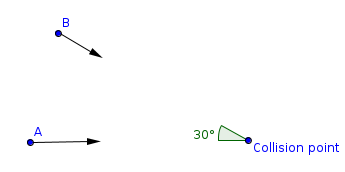
\includegraphics[width=0.4\textwidth]{collision}

            The two cars collide and stick together, moving off together as one unit with speed \SI{1.932}{\metre\per\second}.
    \begin{parts}
      \part Draw a vector diagram depicting the conservation of momentum.
      \part Car $ A $ was originally travelling at a speed of \SI{1.67}{\metre\per\second}. What was the initial speed
            of car $ B $?
      \part Show that the collision was inelastic (i.e. kinetic energy was \textbf{not} conserved).
    \end{parts}
  \question \textit{Projectiles.} A tennis ball is fired from the roof of a \SI{10}{\metre} tall building at an angle of \SI{20}{\degree} to the
            horizontal with an initial velocity of \SI{20}{\metre\per\second}.
    \begin{parts}
      \part Explain in detail what assumptions we make in order to model the ball as a projectile, and justify whether these assumptions are reasonable.
      \part Calculate the following:
        \begin{itemize}
          \item The maximum height above the ground reached by the ball.
          \item The vertical speed with which it is travelling when it hits the ground.
          \item The time taken to hit the ground.
          \item The range of the ball (i.e. the horizontal distance it travels before it hits the ground).
        \end{itemize}
    \end{parts}
\end{questions}

\vspace*{\fill}
This version: \today

\end{document}
